\documentclass[11pt,a4paper]{article}
\usepackage{amsmath,amsthm,amsfonts,amssymb,amscd}
\usepackage{enumerate} 
\usepackage{physics}
\usepackage{enumerate}
\usepackage{fancyhdr}
 \usepackage{hyperref}
\hypersetup{colorlinks,
    linkcolor=blue,
    citecolor=blue,      
    urlcolor=blue,
}
\usepackage{graphicx}


\oddsidemargin0.1cm 
\evensidemargin0.8cm
\textheight22.7cm 
\textwidth15cm \topmargin-0.5cm

\newtheorem{theorem}{Theorem}[section]
\newtheorem{lemma}[theorem]{Lemma}

\usepackage{listings}
\usepackage{xcolor}

\definecolor{codegreen}{rgb}{0,0.6,0}
\definecolor{codegray}{rgb}{0.5,0.5,0.5}
\definecolor{codepurple}{rgb}{0.58,0,0.82}
\definecolor{backcolour}{rgb}{0.95,0.95,0.92}

\lstdefinestyle{mystyle}{
    backgroundcolor=\color{backcolour},   
    commentstyle=\color{codegreen},
    keywordstyle=\color{magenta},
    numberstyle=\tiny\color{codegray},
    stringstyle=\color{codepurple},
    basicstyle=\ttfamily\footnotesize,
    breakatwhitespace=false,         
    breaklines=true,                 
    captionpos=b,                    
    keepspaces=true,                 
    numbers=left,                    
    numbersep=5pt,                  
    showspaces=false,                
    showstringspaces=false,
    showtabs=false,                  
    tabsize=2
}

\lstset{style=mystyle}

\newcommand{\silvia}[1]{{ {\color{blue}{(silvia)~#1}}}}
\newcommand{\grace}[1]{{ {\color{purple}{(grace)~#1}}}}

\pagestyle{fancy}
\fancyhf{}
\lhead{\textsc{Open DP Privacy Proofs: Measurements (Is Equal)}}
\renewcommand{\headrulewidth}{0pt}
\begin{document}

\vspace{0.2cm}
\emph{Written by Grace Tian}
\vspace{0.2cm}

% \section{Cast}

\section{Is Equal} 
Lines 40-56 of \url{https://github.com/opendp/opendp/blob/21-impute/rust/opendp/src/trans/cast.rs#L40-L56}

\subsection{Code}

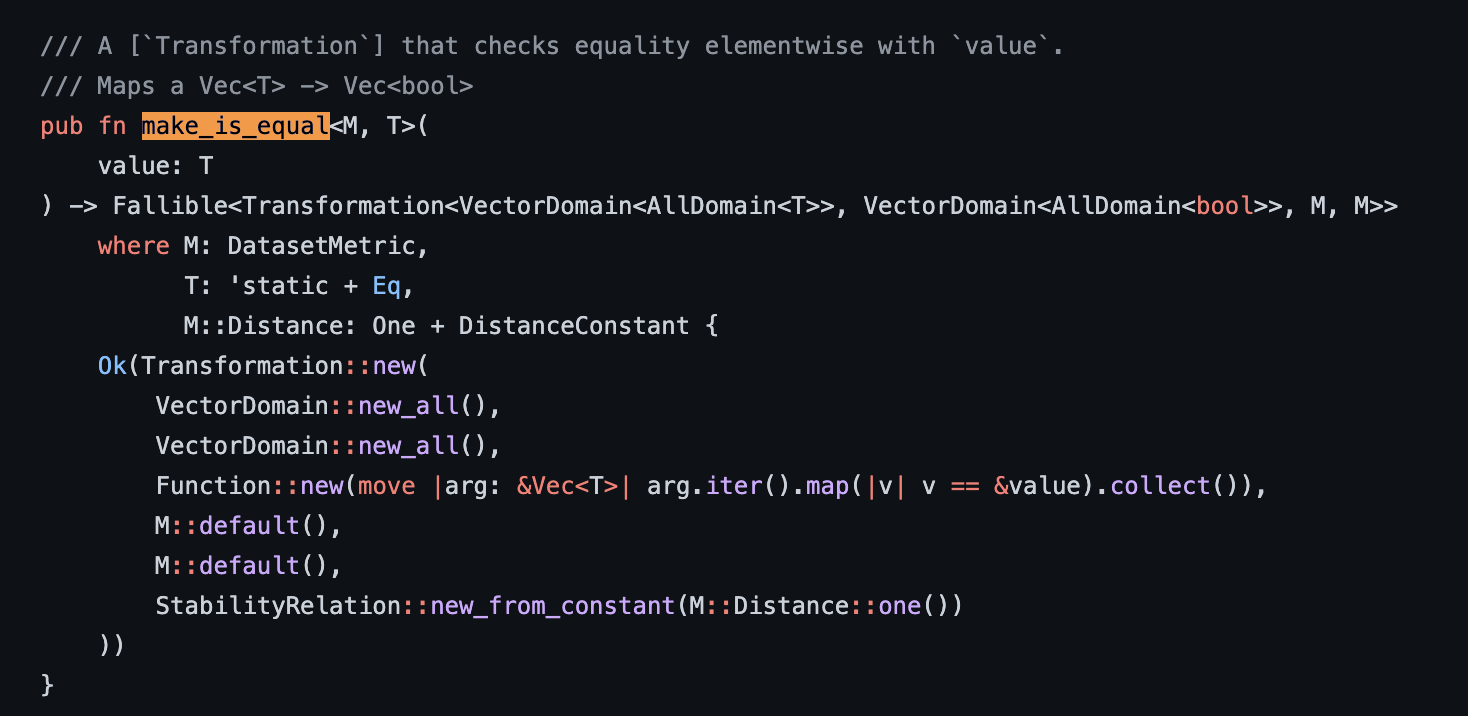
\includegraphics[width=\textwidth]{make_is_equal.png}


\subsection{Pseudo Code}
% \silvia{I think perhaps it is useful to include the function as an equation}

\begin{lstlisting}[language=Python]
def make_is_equal(value : T, metric):
    input_domain = (VectorDomain(AllDomain(T));
    output_domain = (VectorDomain(AllDomain(bool));
    input_metric = metric; 
    let output_metric = metric
    assert is_instance(metric, SymmetricDistance);
    
    let function(data: Vec<T>) -> Vec<Bool>: 
        return map(data == value);
    let stability_relation = lambda(d_in, d_out): (d_in <= d_out);
    
    return Transformation(input_domain, output_domain, function, input_metric, output_metric, stability_relation)

Is_Equal = make_is_equal(value, SymmetricDistance);
\end{lstlisting}


\subsection{Conditions as Specified in Pseudo Code}
\begin{itemize}
    \item Input Domain: all vector domain of input value type \texttt{T} (same type as input \texttt{value}). T is a generic type that is static and can be evaluated with equality.
    \item Output Domain: all vector domain of type \texttt{bool}.
    \item Function: returns vector mapping of whether vector elements equal input \texttt{value}.
    \item Input Metric: Symmetric Distance
    \item Output Metric: same as Input Metric. 
    \item Stability Relation: function that takes in 32 bit integers $d_{in}$ and $d_{out}$ and returns whether $d_{in} \leq d_{out}.$
\end{itemize}

\silvia{Do we need to include the stability parameter? And perhaps include an example calling \texttt{make\_is\_equal} with metrics?}

\silvia{Shouldn't it be checked / imposed that the end user passes the same input and out metric somewhere? Otherwise have only one?}

\subsection{Proof}

\begin{theorem}
For every setting of the input parameters to \texttt{make\_is\_equal}, the transformation returned by \texttt{make\_is\_equal} has the following properties
\begin{enumerate}
    \item \textup{(Appropriate output domain).} If vector \texttt{v} of type \texttt{T} is in the input domain, then \texttt{function(v)} is in the output domain, otherwise the program will raise an \texttt{Exception}. 
    \item \textup{(Stability Guarantee).} If two vector inputs $v, w$ are "$d_{in}$ - close" and if \texttt{Relation($d_{in}$, $d_{out}$) = True} then the corresponding outputs $function(v), function(w)$ are "$d_{out}$ - close". 
\end{enumerate}
\end{theorem}
\begin{proof}
\begin{enumerate}
\item \textup{(Appropriate output domain).} Rust automatically enforces the type system to ensure it is in the correct output domain. The type signature of the function in the pseudo code and Rust code takes in a \texttt{Vec<T>} and returns \texttt{Vec<Bool>}. Since the rust code successfully compiles, by definition of the type signature the theorem must hold. Otherwise, the code will raise an exception for incorrect input type.



\item \textup{(Stability Guarantee).}
We can assume $d_{in} \leq d_{out}$ because Relation($d_{in}$, $d_{out}$) = \texttt{True}. We consider the symmetric distance as input metric. Since vector inputs $v, w$ are $d_{in}$-close, then by definition the symmetric distance of the multisets is bounded by $d_{in}$: $\abs{MultiSet(v) \Delta MultiSet(w)} \leq d_{in}$ 

% We can denote the histogram of the multiset $v \in MultiSets(\mathcal{X})$ as $h_v : \mathcal{X} \to \mathbb{N}$ where $h_v(z)$ is the number of occurrences of $z$ in $\mathcal{X}$. $$d_{Sym}(v, w) = \norm{h_v - h_w}_1 = \sum_{z} \abs{h_v(z) - h_w(z)}.$$

We want to show that $\abs{MultiSet(function(v)) \Delta MultiSet(function(w))} \leq d_{out}$. %\\$\abs{MultiSet(function(v))\Delta MultiSet(function(w))} = \norm{h_{is\_equal(v)} - h_{is\_equal(w)}}_1 \leq d_{out}$. 
To do so, we consider the symmetric distance between the multiset transformations $function(v)$ and $function(w)$. We claim that for any pair of set elements $v^* \in Multiset(v)$ and $w^* \in Multiset(w)$ $$\abs{MultiSet(function(v)) \Delta MultiSet(function(w))} \leq \abs{MultiSet(v) \Delta MultiSet(w)}$$
We consider 4 cases. 
\begin{itemize}
    \item WLOG $v^* ==$ \texttt{value}, $w^* \neq \texttt{value}$ \\
    When we apply the \texttt{function()} to the elements, we will still get different values (\texttt{T} and \texttt{F}). So the symmetric distance stays the same after we transform 2 sets with these elements separately.
    
    \item $v^* == $ \texttt{value}, $w^* == $ \texttt{value} \\
    When we apply the \texttt{function()} to the elements, we will still get same values (\texttt{T} and \texttt{T}). So the symmetric distance stays the same after we transform 2 sets with these elements separately.
    
    \item $v^* \neq $ \texttt{value}, $w^* \neq $ \texttt{value} \\
    When we apply the \texttt{function()} to the elements (which are not necessarily the same), we will get the same values (both \texttt{F}). So the symmetric distance must nonstrictly decrease after we transform 2 sets with these elements separately.
    
\end{itemize}

Since we considered all possible pairs of elements, the symmetric distance must nonstrictly decrease after we transform 2 multi sets $v$ and $w$. 

$$\abs{MultiSet(function(v)) \Delta MultiSet(function(w))} \leq \abs{MultiSet(v) \Delta MultiSet(w)}$$ Since the right hand side $\leq d_{in} \leq d_{out}$, then the transformed outputs are $d_{out}$-close: $\abs{MultiSet(function(v)) \Delta MultiSet(function(w))} \leq d_{out}$.

\end{enumerate}
\end{proof}

\silvia{I think you are using the histogram notation implicitly because I don't think you can say something like $function(v) = T$ (for true) because it is a vector/set, and you mean to say one entry, right? } \grace{Not super sure - it's just function applied to a singular element $v$ but that's not a vector of size 1.} \silvia{Ah then it is the map we discussed today}

\end{document}
